\documentclass[tikz]{standalone}

\usepackage[T1]{fontenc}
\usepackage[english]{babel}

\begin{document}
	\begin{tikzpicture}
		\node[visible on=<1-2>] (dsm) at (0,0) {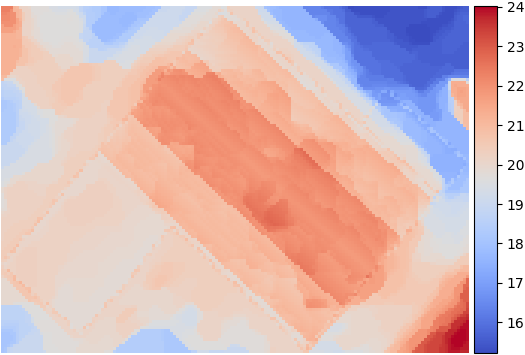
\includegraphics[width=3cm]{images/features/height/dsm-292034}};
        \path (dsm.south) node[anchor=north, text width=3cm, align=center, visible on=<1-2>] (dsm_legend) {\scriptsize \acrshort{acr::dsm}};

        \path (dsm.east) node[anchor=west, visible on=<2>] (minus) {\Large --};

		\path (minus.east) node[anchor=west, visible on=<2>] (model) {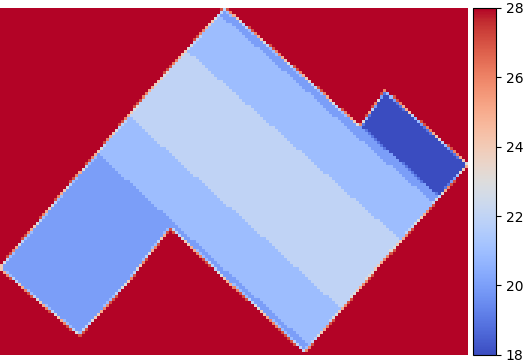
\includegraphics[width=3cm]{images/features/height/heightmap-292034}};
        \path (model.south) node[anchor=north, text width=3cm, align=center, visible on=<2>] (model_legend) {\scriptsize Model heights};

        \path (minus) node[visible on=<3>] (residual) {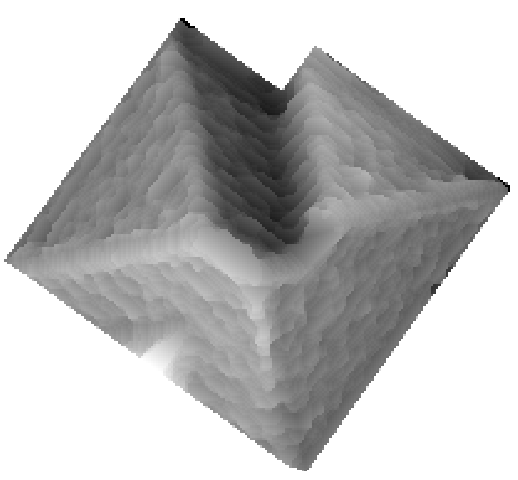
\includegraphics[width=3cm]{images/features/scatnet/residual}};
        \path (residual.south) node[anchor=north, text width=3cm, align=center, visible on=<3>] (residual_legend) {\scriptsize Residuals};

        \path (residual.west) node[anchor=east, visible on=<3>] (equals) {\Large =};

	\end{tikzpicture}
\end{document}
